\begin{figure*}
  \centering
  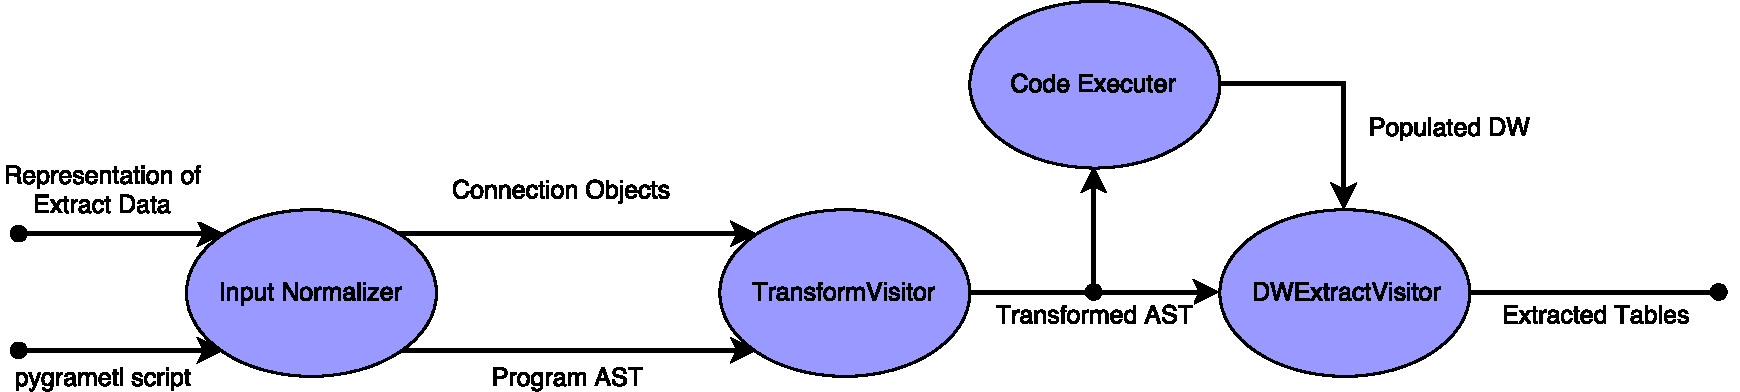
\includegraphics[width=1\textwidth]{figures/reinterpreter_model.pdf}
  \caption{Model of our Reinterpreter}
  \label{fig:reinterpreter}
\end{figure*}

\section{pygrametl Reinterpreter}
With  \FW{} we want testing to be as easy as possible. Users should not need to  change their ETL system when testing. To support this, \FW{} takes as input a pygrametl program and a set of mappings between user-defined test data and data sources found in the program. It is important that test data can be used, as actual data from live systems may be off limits to testers. Furthermore, as dummy DW also needs to be given to \FW{}, as testers might again not have access to the real DW. Once specified, \FW{} will run the pygrametl program using the test data and populating the dummy DW. The resulting populated dummy DW can then be extracted and used in user specified test predicates. To acheive the specified goal, we must answer the following four subproblems: 

\begin{itemize}
\item How should users specify their inputs, and how do we normalize it?
\item How do we transform the pygrametl program to use these input?
\item How do we execute the transformed pygrametl program?
\item How do we extract the resulting DW, and how is this data represented? 
\end{itemize}

For \FW{} we implement a component, which we call a reinterpreter. A data flow model describing this component can be seen in \cref{fig:reinterpreter}. Each object that the data flows through represent a solution to one of the subproblems. The reinterpreter is able to take as input different kinds of test data, such as list of dictionaries or a database connection. The \textit{InputNormalizer} then makes sure to represent all test data in a uniform way, so that it is easier to handle. The object also parses the pygrametl program, generating an AST. The \textit{TransformVisitor} then changes the AST of the given pygrametl program, replacing source data with test data. Afterwards the \textit{CodeExecuter}, executes the transformed program , thus populating the DW. Lastly the \textit{DWExtractVisitor} extracts the different tables from the DW, by using schema information residing in the transformed AST. In the following subsections, we will look into each of these four objects and their implementations.

\subsection{InputNormalizer}
\todo[inline]{NOT YET IMPLEMENTED: THIS IS SOME DRAFT STUFF}
The \textit{InputNormalizer} has three main functionalities: it parses the pygrametl program generating an AST, it supplies variables names to the \textit{TransformVisitor} and it has to build a scope for the \textit{CodeExecuter}.

 Parsing is done using the default python package, \texttt{ast}. This however limits us to only reinterpreting pygrametl scripts that contains all the necessary information required for later use.

We would like to support as many representations of source  data for the ETL process as possible. And as such, bla blah blaah. \todo[inline]{Når vi engang har implementeret InputNormalizeren, så skriv lidt om hvordan den fungere her. Det tænkes at den bliver modulær og nok bruger noget dependency injection. Sådan at man nemt kan tilføje flere måder at give Extract Data på}


\subsection{TransformVisitor}
The \textit{TransformVisitor} transforms the pygrametl program by changing nodes in ithe generated AST. It has two main functionalities: changing the program so it generates a DW from test data, and ensuring that connection to the DW is not closed prematurely.  

For the first functionality,\textit{TransformVisitor} locates instantiations of pygrametl datasource objects on the AST of the program. For each object, its connection parameter is switched out with a variable name set by the \textit{InputNormalizer} that points to an appropriate test data object. This way, whenever these sources are used in the future, they will connect to and use the user specified data. For the second functionality, we ensure that the connection to our DW is never closed. If we find a statement that does this. we delete it from the AST. This is done as we need to use this connection later on in the \textit{DWExtractVisitor}, when the populated DW needs to be accessed. 

\subsection{CodeExecuter}
The \textit{CodeExecuter}'s only function is to execute the transformed AST it recieves from the \textit{TransformVisitor}. It does this by compiling the AST using the build-in python function \texttt{compile()}, and then executing the compilation using the build-in function \texttt{exec()}. The test data objects are imported into the scope of the program for the execution, so that the refferences inserted by\textit{CodeExecuter} point  to the data. This is done by giving a dictionary that maps references to tests data, as the \texttt{locals} parameter to the \texttt{exec()} function. Executing the transformed pygrametl program in this way then results in the population of the DW.

\subsection{DWExtractVisitor}
The \textit{DWExtractVisitor} builds a representation of the data found in the populated DW, so that it can be used in the user-defined test predicates. The component connects to the DW through the connection we left open in the \textit{TransformVisitor}. It then builds a \textit{DimRepresentation} and \textit{FTRepresentation} for each Dimension and FactTable instantiation in the pygrametl program. It gathers information about table name and attributes from said instantiations. This does limit our users to only be able to instantiate their Dimensions and FactTables using hardcoded string values. As we cant extract the value of a variable through an AST. \todo[inline]{Vi har allerede kørt programmet på det her tidspunkt, kan vi ikke bare gemme Dims og FTs og så hente de værdier ud der. I stedet for at bruge AST'en. Dette gør at vi ikke har denne limitation.}

Once the \textit{DimRepresentation}s and \textit{FTRepresentation}s have been made, they are concatenated into the collection class \textit{DWRepresentation}. This can then later be used by the predicates.

\subsubsection{DWRepresentation}
\todo[inline]{Skrive lidt om hvorfor vi laver DWRep og hvad den indeholder}
